% !TeX root = ../main.tex

\chapter{基于事件相机的火焰检测算法}
在前面的章节里,我们介绍了本次工作数据集的构建,介绍了对数据集图像的相关处理以及特征的提取。这一部分,
我们将在上述工作的基础上,利用支持向量机,通过机器学习的方法思路,搭建并训练一个较完善的火焰检测模型。
我们将利用这个模型,初步对有火和无火图象场景进行分类测试,并对其测试效果进行评价与比较。

\section{感兴趣区域(ROI,region of interest)提取}
在训练模型前,我们要对图像的可疑区域,也就是存在疑似火焰的事件区域进行提取,这一工作,我们将按照以下步骤进行。

步骤一:将事件按照一定的时间间隔(33ms)取样投影到平面上,形成二维事件帧图象。这里的思路与第四章中提取还原部分
类似,不再详细介绍,自行参考。主要流程是将33ms的全部事件按照其空间坐标,投影到二维的像素平面上,形成事件云(点云)。
接着,通过选择合适的参数进行膨胀和腐蚀操作,将周围的噪声去掉,只留下一定大小的事件团。

效果图可参考第四章。

步骤二:采用 Suzuki85 算法完成封闭图形的边缘检测。

Suzuki85 算法是一种著名的轮廓跟踪算法\cite{suzuki1985topological},许多图像处理库(例如 OpenCV)都使用这种边界跟踪算法来进行图像的拓扑结构分析。
这是最早定义边界之间层次关系的算法之一。该算法还区分外边界或孔边界,在图像处理中,外边界指的是对象的外轮廓或边缘,即
对象与背景之间的分界线。外边界检测是图像分割和特征提取的重要步骤之一,常用的算法包括边缘检测算法(如Sobel、Canny、Prewitt等),
用于找到图像中对象与背景之间的明显边界;孔边界指的是对象内部的空洞或孔洞的边界,也称为内边界。孔边界的检测和处理通常涉及到图像的
填充或闭合操作,以消除对象内部的孔洞,从而更好地识别和分析对象的形状和结构。如图\ref{17}所示,B1,B3就是外边界,B2就属于孔边界。
\begin{figure}[ht]
    \centering
    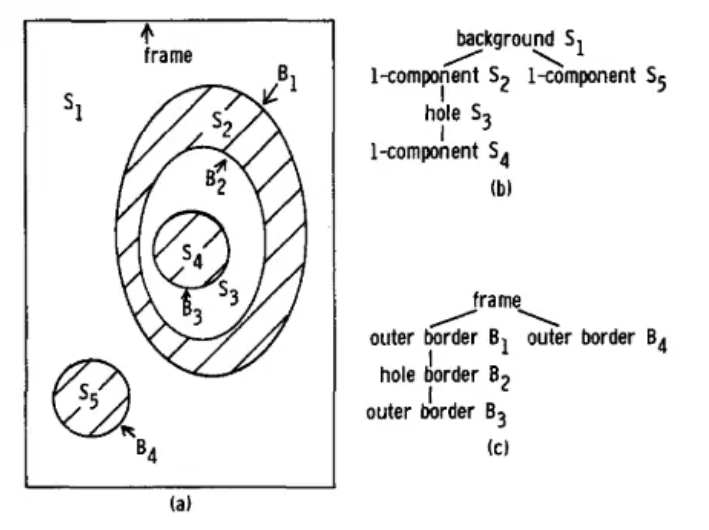
\includegraphics[width=\textwidth]{figures/algorithm_boundary.png}
    \caption{孔与边界示意图}
    \label{17}
\end{figure}

假设$f_{i,j}$表示位置(i,j)处的像素值,图片的最上行、最下行、最左列和最右列组成了它的框架。在此,我们为找到的每个新边界分配一个唯一的编号,并用NBD表示。
我们假设帧的 NBD 为 1。其余边界按顺序编号。我们将任何边界的父级信息保存在 LNBD 或最后一个 NBD 中。

算法开始,从左到右扫描图像,直到找到对象像素。确定它是外边界还是孔边界。检查外边界或孔边界的标准如下图所示。这样在扫描时如果发现如下图\ref{18}所示的情况,我们就可以很容易判断出它是外边界的起点(a)还是孔边界的起点(b)。
\begin{figure}[ht]
    \centering
    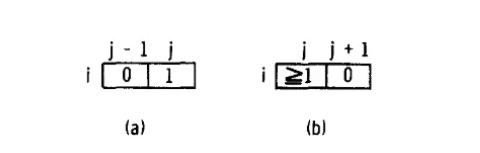
\includegraphics[width=\textwidth]{figures/algorithm_condition.png}
    \caption{判断条件}
    \label{18}
\end{figure}


仅对 >0 的像素执行以下步骤。每次我们开始扫描新行时,将 LNBD 重置为 1。

第一步:

1.如果它是外边界(即$f_{i,j}=1$且$f_{i,j-1}=0$),则增加 NBD 并将$(i_2,j_2)$设置为(i,j-1)

2.否则,如果它是孔边界,则增加 NBD。将$(i_2,j_2)$设置为(i,j+1)并且在$f_{i,j}>1$的情况下 LNBD = $f_{i,j}$

3.否则,转至步骤 3。

第二步:现在,从这个起点,我们将追踪边界。这可以完成为

1.从$(i_2,j_2)$开始顺时针环顾邻域的像素,找到一个非零像素并将其表示为$(i_1,j_1)$,如果没有找到非零像素,则设置$f_{i,j}=-NBD$ 并转到步骤 4。

2.设$(i_2,j_2)=(i_1,j_1)$且$(i_3,j_3)=(i,j)$

3.从像素$(i_2,j_2)$的下一个元素开始,按逆时针方向,再次逆时针方向遍历$(i_3,j_3)$的邻域,找到第一个非零像素,并将其设置为$(i_4,j_4)$。

4.将当前像素$(i_3,j_3)$的值按照下列规则更改:如果$(i_3,j_3+1)$处的像素是属于边界外区域的0像素,则将当前像素值设置为-NBD;
如果$(i_3,j_3+1)$处的像素不是 0 像素且当前像素值为 1,则将当前像素值设置为 NBD;否则,不要更改当前像素值。

5.如果在步骤 2.3中,我们再次返回起点,即$(i_4,j_4)=(i,j)$且$(i_3,j_3)=(i_1,j_1)$转到步骤 3。否则,设置$(i_2,j_2)=(i_3,j_3)$和$(i_3,j_3)=(i_4,j_4)$并返回步骤 2.3。

第三步:如果$f_{i,j}!=1$则设置 LNBD =|$f_{i,j}$| 并从下一个像素(i,j+1)开始扫描。当我们到达图像的右下角时,算法停止。

图\ref{19}中逐步展示了Suzuki85算法进行一次迭代的示例。
\begin{figure}[ht]
    \centering
    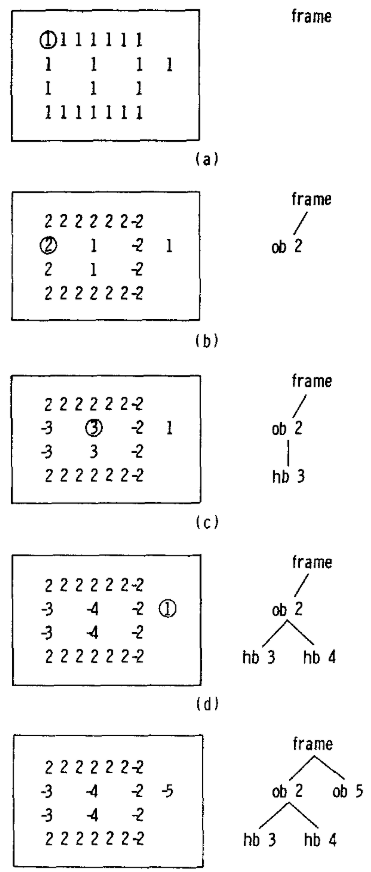
\includegraphics[width=0.49\textwidth]{figures/algorithm_example.png}
    \caption{迭代示例}
    \label{19}
\end{figure}

步骤三:利用并查集算法(Union Find Algorithm),以余弦相似度作为指标,融合相似的边缘,获得最终的感兴趣区域。

并查集算法是一种用于处理集合合并与查找问题的数据结构和算法。它主要用于解决一些元素分组的问题,例如连通性问题、集合合并问题等。

并查集算法的主要流程如下:

1.初始化(MakeSet):将每个元素初始化为一个单独的集合,每个集合中只包含一个元素。

2.查找(Find):查找元素所属的集合,通常用于确定两个元素是否属于同一个集合。这个操作通常伴随着路径压缩以优化查找速度。

3.合并(Union):合并两个集合,通常将两个集合的代表元素(或根节点)连接起来,从而将它们合并成一个更大的集合。

并查集通常用一个数组来表示集合,并通过一些技巧实现上述操作:

1.集合数组:用于存储每个元素所属的集合。初始化时,每个元素的父节点指向自己,表示它们都是独立的集合。

2.路径压缩:在查找操作中,将查找路径上的每个节点都直接连接到根节点,从而优化后续查找操作的速度。

3.按秩合并:在合并操作中,通过维护每个集合的秩信息,使得合并后的树更加平衡,从而减少查找的时间复杂度。

并查集算法的时间复杂度通常为 O(α(n)),其中 α(n) 是阿克曼函数的反函数,增长速度非常缓慢,因此并查集算法通常被认为是高效的。

余弦相似度是一种用于比较两个向量之间相似度的度量方法,常用于信息检索、自然语言处理、推荐系统等领域。它衡量的是两个向量在多维空间中的夹角的余弦值,其取值范围在[-1, 1]之间。

假设有两个向量 A 和 B,它们的余弦相似度 sim(A,B) 可以通过以下公式计算:
\begin{equation} 
    sim(A,B)=\frac{A·B}{\lVert A \rVert \lVert B \rVert}
\end{equation}

其中,A·B是两个向量的内积,$\lVert A \rVert$和$\lVert B \rVert$分别是两个向量的范数。余弦相似度的值越接近1,则表示两个向量越相似;值越接近-1,则表示两个向量越不相似;值为0则表示两个向量之间没有相关性。
这里我们在进行并查集的集合合并时,便是利用余弦相似度来衡量其相似度,进行合并操作。


\section{基于SVM的ROI区域训练}
\subsection{样本制作}
SVM接收的数据是由第四章中提取的的火焰静态和动态特征所组成的高维向量[a,b,c,d,···],后面我们统一称它为FIRE向量。
从多次初步实验的效果出发,我们发现FIRE向量的维度越高,分类的效果会出现正相关变化,但随着维度增加,后续的提升也会越来越不明显。
出于效率和效果的双重考虑,我们的FIRE向量样本制作定为7个维度,并根据实际的有无火焰的区分效果,选择了7个区分度较为明显的动态和静态特征,接下来将一一介绍。

1.事件输出率。我们在第四章的静态特征部分已经详细介绍讨论过它的定义,此处便不再累述。简而言之,我们此处使用的
事件输出率即为采样时间段内触发事件总数与标准采样间隔的比值(33ms)。事件输出率数值越大,越可能是疑似的火焰区,该维可用于区分与火焰事件输出频率差距较明显的干扰源。

2.长宽比。这是图像学里比较经典的特征,可以呈现一定的火焰形状特征。我们是利用Suzuki85 算法,做出初步的事件追踪框,对框中密集事件团的长宽比进行计算。

3.圆形度。圆形度表征的是火焰轮廓与圆形的相似度,同样在第四章中介绍,用于区分一般有着较高圆形度的规则外界物体。

4.矩形度。与圆形度相似,火焰越不稳定该数值越高,用于和圆形度配合区分外界规则物体。

5.尖角数。尖角是火焰动态识别中最重要的特征,在第四章的动态特征中也花了较多的篇幅来介绍,我们是利用Harris角点检测算法检测
33ms图像中的角点来进行的。该项特征可以效果较为显著的区分火焰与大部分的非火焰干扰源,属于本次火焰识别工作中的最优特征。

6.火焰生长系数。在第四章也有介绍,这是火焰发展阶段中的一个重要特征,我们这里的处理方法是将33ms的事件帧图象再度划分为三个11ms,对每组的3幅时间图像按照定义进行
生长系数的计算。

7.火焰形心偏移。我们在第四章介绍了火焰形心的移动特性,这里我们的处理也是将其每组划分为3幅11ms图象,通过统计每幅图像的面积,矩,形心坐标,从而
计算出由第一个11ms到第三个11ms,事件图像形心的移动距离,由于取样间隔自始至终一致,该数值可以一定程度上反映形心的位移速度(位移与微小时间间隔取比值),从而反应
运动特性。该项特征可以较好区分外界规则运动干扰源(如移动发光体,行人等)。

其余我们在第四章中还介绍了很多特征,未能选用都是出于效果或效率考虑,例如火焰的频闪特性区分效果极差,高阶矩的计算较为繁琐。
\subsection{样本训练}
我们将数据集划的事件帧序列,按照上述的制作方法,每一帧都转化为一条七维的FIRE向量,我们根据之前标定的数据集
标签(有无火焰),将这些向量分为正样本(有火)和负样本(无火)。划分完毕后,为了使训练模型的效果最佳,我们后面后续实验中训练集和测试集
正样本和负样本数量均大致保持1:1的比例,其中每次实验约600组数据作为训练集,随机抽取4000组作为测试集。
\subsection{核函数的确定}
对于SVM的模型训练来讲,核函数的选择至关重要,它可以将原始数据通过非线性映射转换为更高维度的特征空间,从而在该空间中实现线性分离,直接关系到模型的效果等各个方面。
SVM常见的核函数有线性核,多项式核,高斯核(RBF),sigmoid核,根据其适用场景和效果,本次工作我们主要涉及使用到线性核linear和高斯核rbf。

线性核函数是支持向量机中最简单的核函数之一。它执行的是一个简单的线性映射,将数据从原始的特征空间映射到更高维的特征空间,但并不引入额外的维度,而是直接在原始的特征空间中进行计算。
线性核函数的数学表达式如下:
\begin{equation} 
    K(x_i,x_j)=x_i^T·x_j
\end{equation}

其中,$x_i$和$x_j$分别表示两个输入样本的特征向量,·表示向量的点积。

线性核函数适用于在原始特征空间中线性可分的情况,即样本可以通过一个超平面将不同类别分开。在这种情况下,使用线性核函数可以直接在原始特征空间中构造一个线性分类器,而无需进行额外的特征转换。
由于我们处理的为二分类问题(有火与无火),在高维的空间内,线性核也可以呈现不错的效果。

高斯核函数,也称为径向基函数核函数,是支持向量机中常用的一种非线性核函数。它将数据映射到无限维的特征空间,并在该空间中进行高斯分布的内积运算。
高斯核函数的数学表达式如下:
\begin{equation} 
    K(x_i,x_j)=exp(-\frac{{\lVert x_i-x_j \rVert}^2}{2\sigma^2})
\end{equation}

其中,$x_i$和$x_j$是输入样本的特征向量,$\lVert x_i-x_j \rVert$表示输入样本之间的欧氏距离,$\sigma$是高斯核函数的一个参数,控制了高斯函数的宽度。

高斯核函数适用于各种类型的数据,无论是线性可分还是非线性可分的情况,都可以通过调节参数来适应不同的数据集。
高斯核函数在特征空间中给予较高权重的区域主要集中在样本附近,因此能够更好地捕捉局部特征。
但是需要注意的是,它的计算复杂度较高,特别是在高维空间中。

我们使用多个不同的干扰源视频,都加入同样的火焰场景,建立一个简单的测试集,对两种核的分类效果进行了一个简单的初步对比,记录如下:多次实验求平均后,linear核的的平均精度在70\%左右,而高斯核(rbf)的平均精度高出linear核约十个百分点,可达到80\%左右;此外,linear核的训练时间远远超过高斯核,速度相差达到三个数量级以上。

可见,在本次工作中处理二分类火焰识别问题上,rbf核目前呈现的效果要明显优于linear核,后面更详细的的实验结果也将佐证这一点。
\section{检测结果}
对SVM训练的火焰检测算法模型进行测试和评估,我们将从检测精度,可视化,检测速度三方面进行展示。
\subsection{检测精度}
目标检测算法的评价指标通常用于评估算法在检测目标位置和类别的准确性、鲁棒性和效率。常见的目标检测算法评价指标包括:

1.准确率(Precision):准确率是指检测出的目标中真正属于目标类别的比例,它衡量了检测结果的精确性。准确率可以通过以下公式计算:
\begin{equation} 
    precision=\frac{TP}{TP+FP}
\end{equation}

其中,TP表示正确检测到的目标数量,FP表示错误地将背景误判为目标的数量。

2.召回率(Recall):召回率是指目标类别中被检测到的比例,它衡量了检测算法对目标的覆盖程度。召回率可以通过以下公式计算:
\begin{equation} 
    Recall=\frac{TP}{TP+FN}
\end{equation}


其中,FN表示未能正确检测到的目标数量。

3.IoU(Intersection over Union):IoU是一种用于衡量目标检测框精确度的指标,它计算检测框与真实目标框之间的重叠程度,根据重叠程度来判断检测框是否达到“正确检测”标准。IoU可以通过以下公式计算:
\begin{equation} 
    IoU=\frac{A\bigcap B}{A\bigcup B}
\end{equation}


4.平均精度均值(mAP):mAP是一种综合评价指标,用于评估检测器在不同类别上的检测性能。它计算每个类别的平均精度(AP),并对所有类别的AP取平均值。

这里,我们将展示linear和rbf两种不同的核的检测精度对比,包括mAP与recall,其中每项指标参数均为三次测试的平均值,且数据为去噪后数据。我们划分了8种情况进行对比:七个FIRE向量全部使用以及七个FIRE向量依次不使用,这样设置的目的一方面可以进行多次的两种核的横向对比,另一方面也可以进行纵向的各向量间接对比,同时这种方式下的情况数较为合适,避免过多排列组合情况造成对比的繁琐复杂。

展示如表\ref{linear},\ref{rbf}。
\begin{table}[ht]
    \centering
    \caption{linear核各情况统计}
    \begin{tabularx}{0.7\textwidth}{c|X|X}
        \toprule
        情况&平均精度均值mAP(\%)&召回率recall(\%)\\
        \midrule
        无事件输出率&77.2&49.4\\
        无长宽比&73.1&47.0\\
        无圆形度&71.1&45.3\\
        无矩形度&71.8&45.4\\
        无尖角数&67.6&42.6\\
        无形心移动&71.0&45.2\\
        无面积生长系数&70.9&45.2\\
        所有FIRE向量&71.9&45.6\\
        \bottomrule
    \end{tabularx}
    \label{linear}
\end{table}





\begin{table}[ht]
    \centering
    \caption{高斯核各情况统计}
    \begin{tabularx}{0.7\textwidth}{c|X|X}
        \toprule
        情况&平均精度均值mAP(\%)&召回率recall(\%)\\
        \midrule
        无事件输出率&77.7&50.1\\
        无长宽比&80.6&52.0\\
        无圆形度&80.6&52.0\\
        无矩形度&80.6&52.0\\
        无尖角数&78.9&51.1\\
        无形心移动&80.6&52.0\\
        无面积生长系数&80.5&51.9\\
        所有FIRE向量&80.6&52.0\\
        \bottomrule
    \end{tabularx}
    \label{rbf}
\end{table}

可以看到各种情况下,无论是mAP还是Recall,高斯核均明显优于linear核,所以本次工作中,高斯核是我们的最优核选择。

接下来我们将展示噪声对本次模型精确度的影响情况,统一选择最优的rbf核,同样设置8种情况,对去噪前后的平均精度均值mAP和召回率Recall进行统计对比。

展示如表\ref{噪前},\ref{噪后}。
\begin{table}[ht]
    \centering
    \caption{去噪前各情况统计}
    \begin{tabularx}{0.7\textwidth}{c|X|X}
        \toprule
        情况&平均精度均值mAP(\%)&召回率recall(\%)\\
        \midrule
        无事件输出率&60.6&43.4\\
        无长宽比&62.2&44.3\\
        无圆形度&62.2&44.3\\
        无矩形度&62.2&44.3\\
        无尖角数&61.4&44.0\\
        无形心移动&62.2&44.3\\
        无面积生长系数&62.1&44.3\\
        所有FIRE向量&62.2&44.3\\
        \bottomrule
    \end{tabularx}
    \label{噪前}
\end{table}


\begin{table}[ht]
    \centering
    \caption{去噪后各情况统计}
    \begin{tabularx}{0.7\textwidth}{c|X|X}
        \toprule
        情况&平均精度均值mAP(\%)&召回率recall(\%)\\
        \midrule
        无事件输出率&77.7&50.1\\
        无长宽比&80.6&52.0\\
        无圆形度&80.6&52.0\\
        无矩形度&80.6&52.0\\
        无尖角数&78.9&51.1\\
        无形心移动&80.6&52.0\\
        无面积生长系数&80.5&51.9\\
        所有FIRE向量&80.6&52.0\\
        \bottomrule
    \end{tabularx}
    \label{噪后}
\end{table}

可以看到,原始噪声对火焰检测识别模型精确度的影响还是较大的,对原始数据进行去噪可以有效提高约20\%的平均精度,对于模型效果的优化来讲至关重要。

\subsection{可视化}
这里,我们将以最直观的方式对模型的效果进行展示。

对于我们训练的模型来讲,最理想的效果便是对火焰进行正确识别分类,如图\ref{20}所示,(a)和(b)分别是对火焰和非火焰的正确分类。其中红色表示目标框,代表着人工标定的真实的结果与标签,蓝色表示预测框,代表我们训练的模型的预测结果。重合度,即计算的IOU越大,代表着我们的这次预测结果越加准确。
\begin{figure}[ht]
    \centering
    \begin{subfigure}{0.49\textwidth}
        \centering
        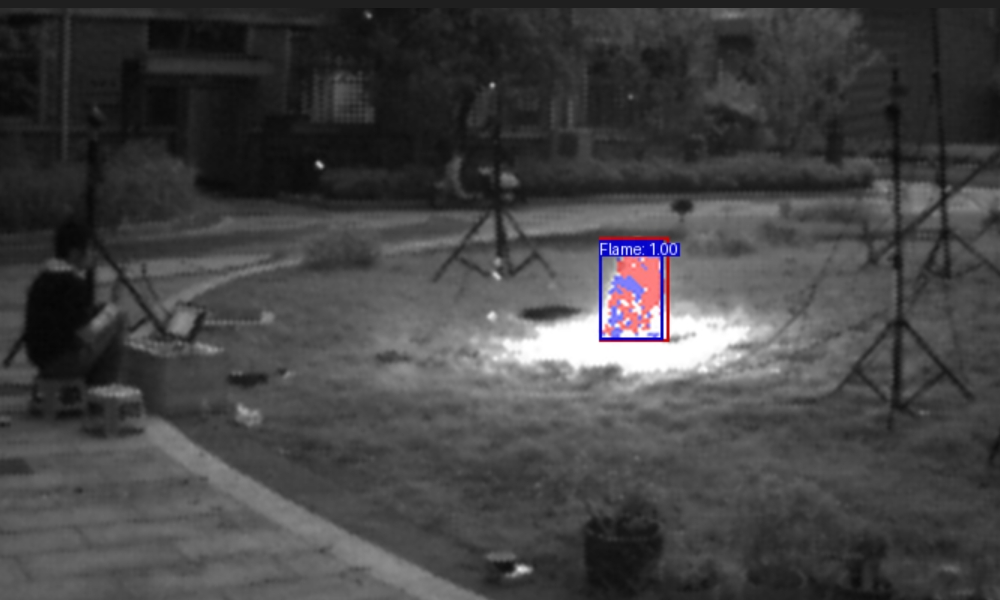
\includegraphics[width=\textwidth]{figures/jiance1.png}
        \caption{火焰识别}
        \label{20.a}
    \end{subfigure}
    \hfill
    \begin{subfigure}{0.49\textwidth}
        \centering
        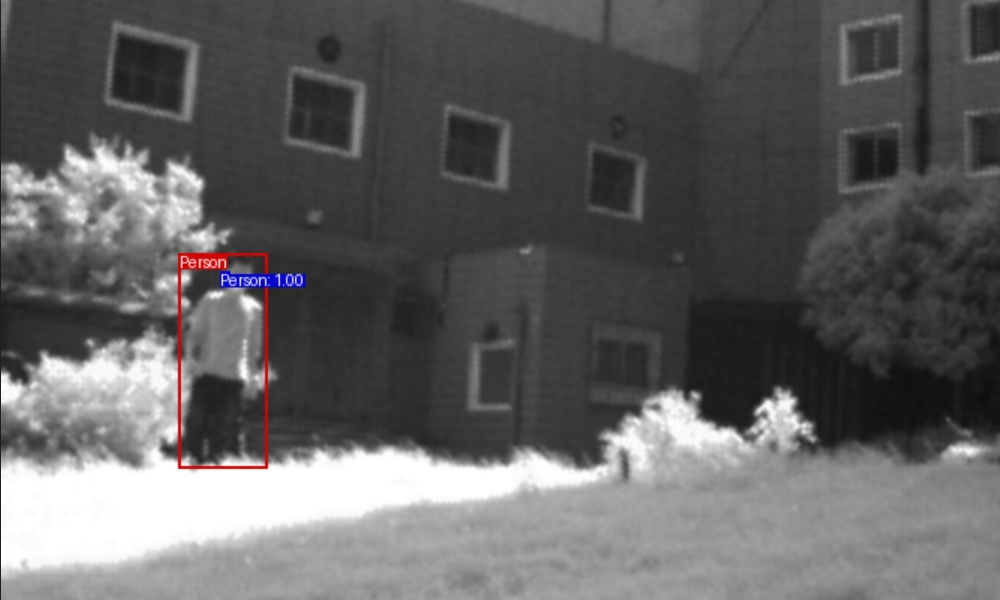
\includegraphics[width=\textwidth]{figures/jiance8.png}
        \caption{非火焰识别}
        \label{20.b}
    \end{subfigure}
    \caption{正确识别}
    \label{20}
\end{figure}
训练的火焰识别模型会出现两类问题,第一类便是将火焰识别成非火焰,从而漏识,如图\ref{21},(a)和(b)分别将火焰错视为行人和夜间的灯光。
\begin{figure}[ht]
    \centering
    \begin{subfigure}{0.49\textwidth}
        \centering
        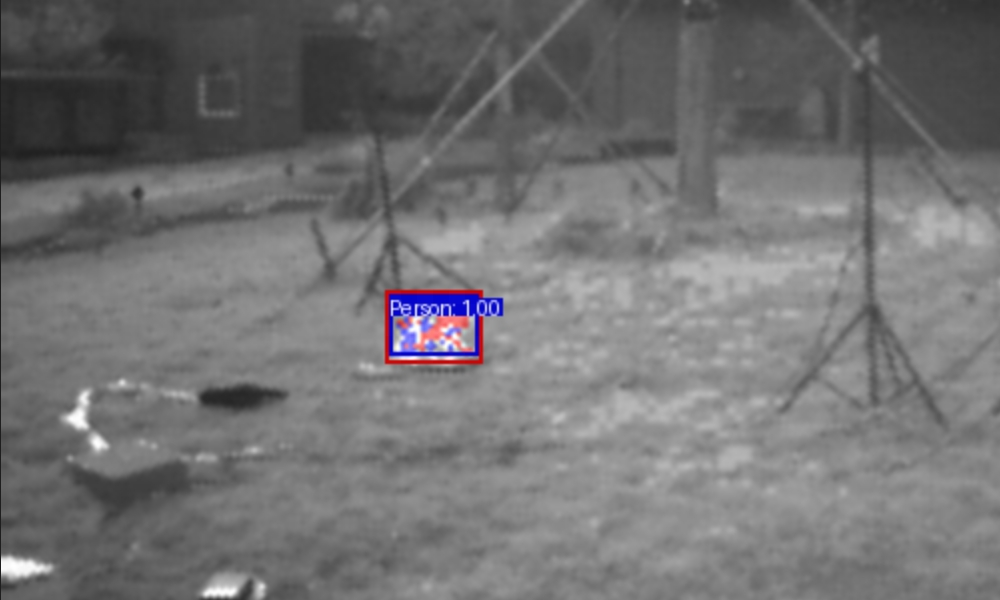
\includegraphics[width=\textwidth]{figures/jiance3.png}
        \caption{错误漏识1}
        \label{21.a}
    \end{subfigure}
    \hfill
    \begin{subfigure}{0.49\textwidth}
        \centering
        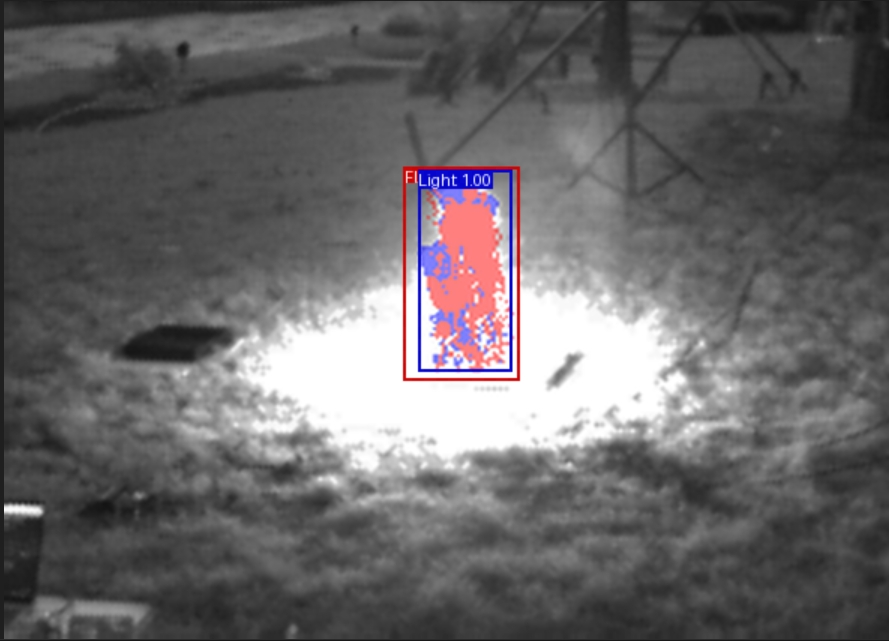
\includegraphics[width=\textwidth]{figures/jiance7.png}
        \caption{错误漏识2}
        \label{21.b}
    \end{subfigure}
    \caption{漏识}
    \label{21}
\end{figure}

漏识情况对于rbf核来讲,出现情况较少,而由于其简单线性结构,linear核相对较多,也是其与高斯核准确度差距的主要所在。我们利用4000组数据对两种核进行了分别测试,高斯核仅仅出现了两例漏识情况,而linear核的漏识会达到200+例。

第二类问题便是将非火焰识别为火焰,从而错误预警,这一问题较为普遍,无论是哪种核函数都相差不大,如图\ref{22}所示,(a)与(b)分别是将运动的行人和夜间的灯光错识别为了火焰。
\begin{figure}[ht]
    \centering
    \begin{subfigure}{0.49\textwidth}
        \centering
        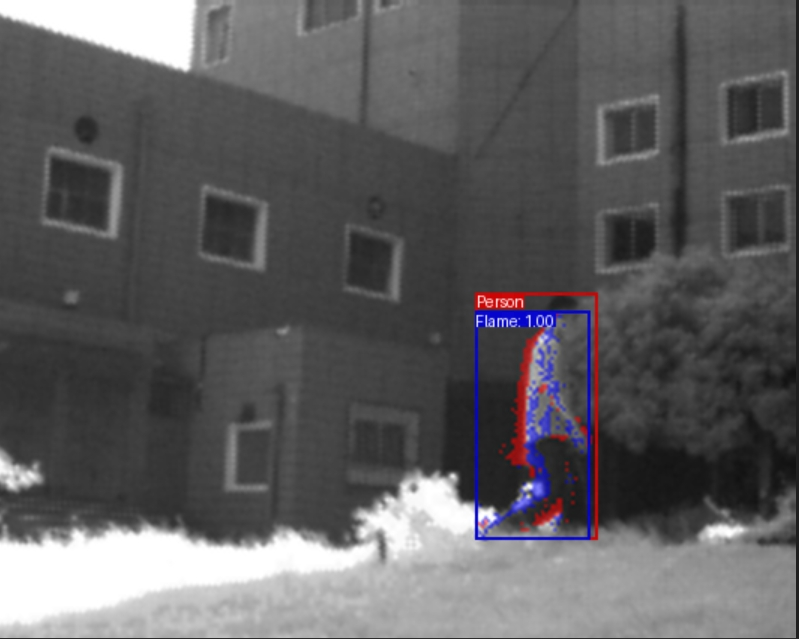
\includegraphics[width=\textwidth]{figures/jiance4.png}
        \caption{错误预警1}
        \label{22.a}
    \end{subfigure}
    \hfill
    \begin{subfigure}{0.49\textwidth}
        \centering
        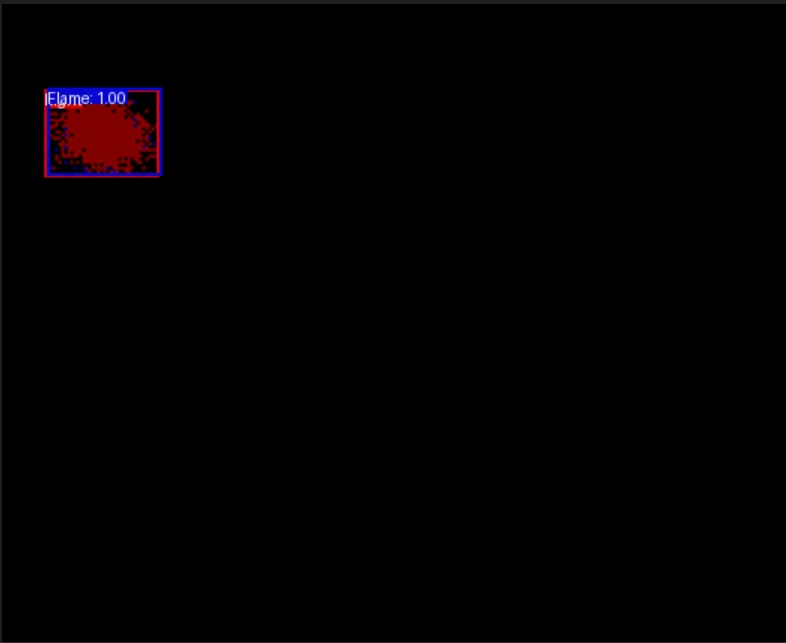
\includegraphics[width=\textwidth]{figures/jiance5.png}
        \caption{错误预警2}
        \label{22.b}
    \end{subfigure}
    \caption{被干扰错误预警}
    \label{22}
\end{figure}

同时该问题会被外界噪声放大,从可视化来看,外界噪声数据会与一些干扰源相连接,从而形成更加与火焰相似的事件团集合,从而更容易被错误预警,而漏识问题反而受噪声影响不大,甚至还会减弱。如图\ref{23}所示,肉眼可见行人的周围事件数据变多,从而被错误预警。
\begin{figure}[ht]
    \centering
    \begin{subfigure}{0.49\textwidth}
        \centering
        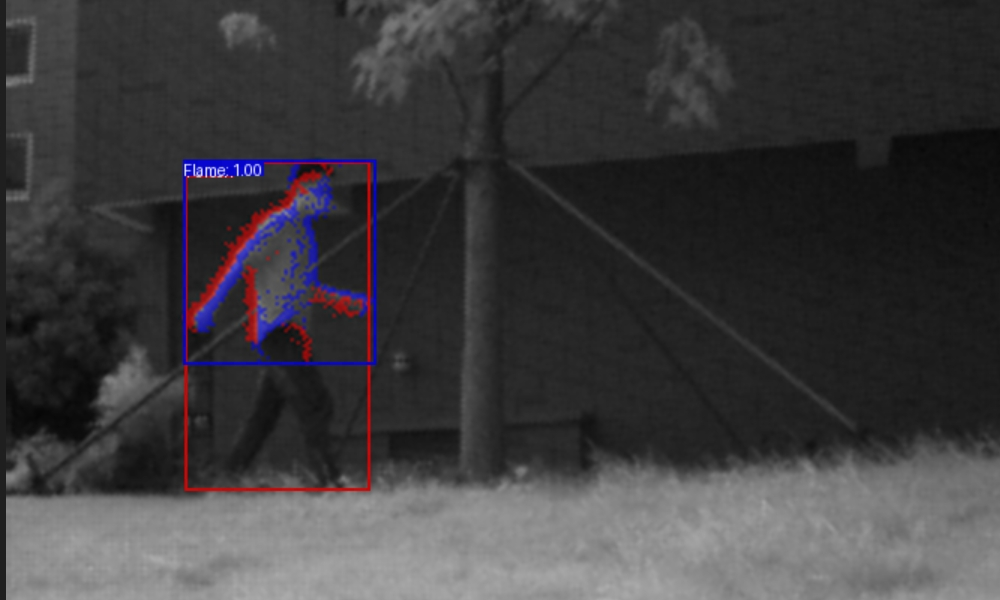
\includegraphics[width=\textwidth]{figures/zaosheng3.png}
        \caption{示例1}
        \label{23.a}
    \end{subfigure}
    \hfill
    \begin{subfigure}{0.49\textwidth}
        \centering
        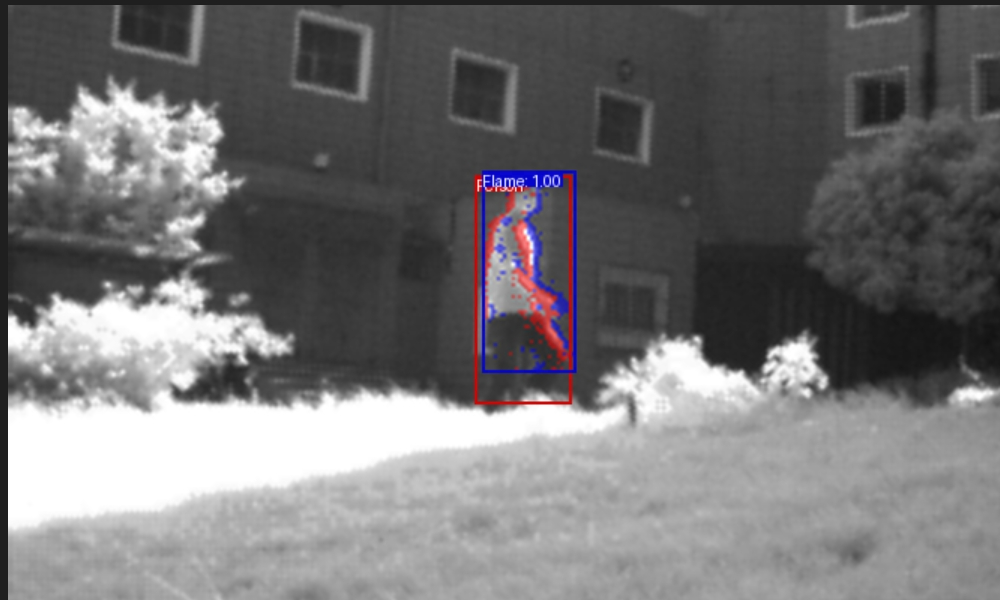
\includegraphics[width=\textwidth]{figures/zaosheng4.png}
        \caption{示例2}
        \label{23.b}
    \end{subfigure}
    \caption{噪声放大错误预警问题}
    \label{23}
\end{figure}

此外噪声还会对正确识别结果产生干扰,由于噪声的存在可能与火焰事件产生连通,从而会使我们模型的预测火焰范围与真实情况相比偏大,这将会影响我们模型的IOU值,从而影响我们根据IOU阈值进行计算的mAP。如果噪声过多,火焰的具体位置也会被剧烈影响。如图\ref{24}所示,(a)即为受噪声影响,预测框偏大的情况,(b)则是更严重的情况,火焰的具体位置被噪声严重干扰。从这一直观角度,去噪对模型效果影响极大。
\begin{figure}[ht]
    \centering
    \begin{subfigure}{0.49\textwidth}
        \centering
        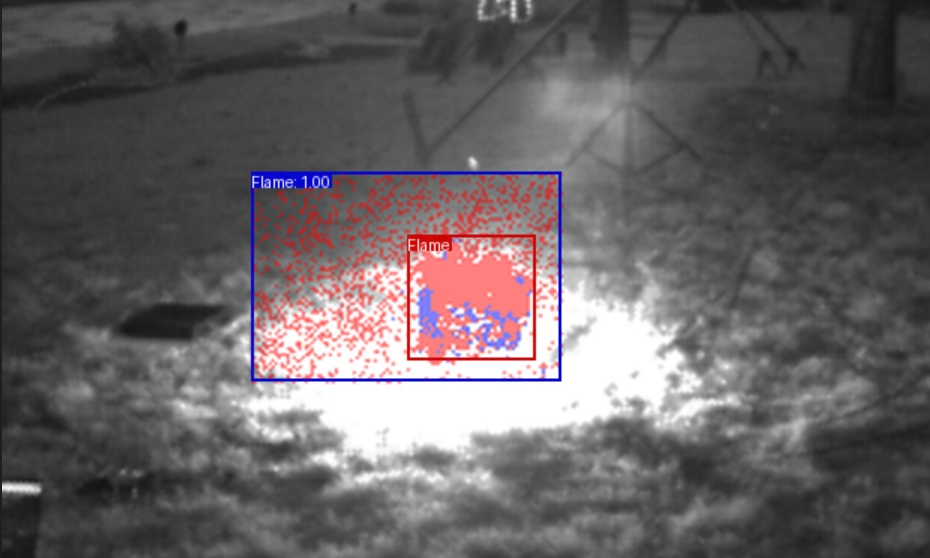
\includegraphics[width=\textwidth]{figures/zaoshen1.png}
        \caption{噪声干扰1}
        \label{24.a}
    \end{subfigure}
    \hfill
    \begin{subfigure}{0.49\textwidth}
        \centering
        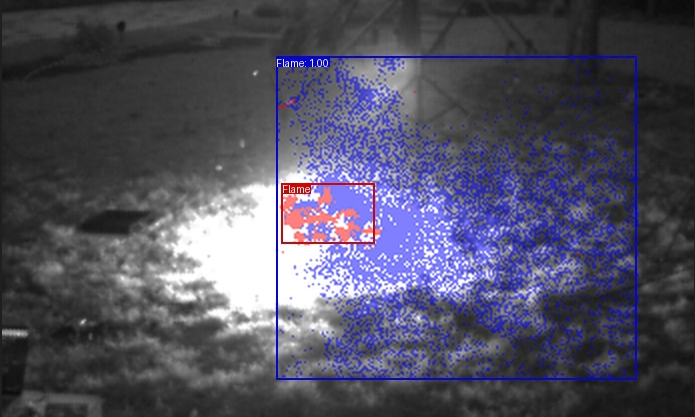
\includegraphics[width=\textwidth]{figures/zaosheng2.png}
        \caption{噪声干扰2}
        \label{24.b}
    \end{subfigure}
    \caption{噪声干扰}
    \label{24}
\end{figure}


\subsection{检测速度}
在前面两部分,我们展示评估了训练的火焰识别模型的准确度等效果方面,然而,效果只是效率的一部分,速率对于模型工作来讲同样重要。这一部分,我们将对该模型的速率进行评估与对比。评估将包括两个指标,训练集的构建时间和模型的训练时间。同样的,我们参照之前,仍然设置8种情况,构建时间和训练时间均是取三次实验的均值。

linear核和高斯核的时间效率情况(数据采用去噪后)统计如表\ref{t_linear},\ref{t_rbf}。
\begin{table}[ht]
    \centering
    \caption{linear核各情况统计}
    \begin{tabularx}{0.7\textwidth}{c|X|X}
        \toprule
        情况&训练集构建时间(s)&火焰检测模型训练时间(s)\\
        \midrule
        无事件输出率&3.62&170.0\\
        无长宽比&3.65&96.2\\
        无圆形度&3.66&51.0\\
        无矩形度&3.66&61.4\\
        无尖角数&3.71&71.2\\
        无形心移动&3.68&73.0\\
        无面积生长系数&3.55&22.0\\
        所有FIRE向量&3.73&69.1\\
        \bottomrule
    \end{tabularx}
    \label{t_linear}
\end{table}



\begin{table}[ht]
    \centering
    \caption{rbf核各情况统计}
    \begin{tabularx}{0.7\textwidth}{c|X|X}
        \toprule
        情况&训练集构建时间(s)&火焰检测模型训练时间(s)\\
        \midrule
        无事件输出率&3.62&0.04\\
        无长宽比&3.63&0.06\\
        无圆形度&3.66&0.06\\
        无矩形度&3.63&0.04\\
        无尖角数&3.71&0.04\\
        无形心移动&3.69&0.04\\
        无面积生长系数&3.57&0.06\\
        所有FIRE向量&3.73&0.04\\
        \bottomrule
    \end{tabularx}
    \label{t_rbf}
\end{table}

由对比可见,由于训练集的构建过程并无差别,两种核的该时间参数几乎保持一致;然而,在训练数据集的所用时间方面,高斯核的速率上与linear有着三个数量级的差距,结合前面的精确度差距,可以说rbf核基本在各方面效率优于linear核。

设置相同的情况,去噪前后的时间速率情况(统一使用rbf核)展示如表\ref{t_噪前},\ref{t_噪后}。
\begin{table}[ht]
    \centering
    \caption{去噪前各情况统计}
    \begin{tabularx}{0.7\textwidth}{c|X|X}
        \toprule
        情况&训练集构建时间(s)&火焰检测模型训练时间(s)\\
        \midrule
        无事件输出率&7.63&0.06\\
        无长宽比&7.85&0.04\\
        无圆形度&8.49&0.04\\
        无矩形度&8.22&0.06\\
        无尖角数&8.40&0.06\\
        无形心移动&8.38&0.06\\
        无面积生长系数&7.60&0.06\\
        所有FIRE向量&8.65&0.04\\
        \bottomrule
    \end{tabularx}
    \label{t_噪前}
\end{table}



由对比可见,由于rbf核模型的训练速率较快,去噪前后的训练时间并无过大变化,属于正常波动变化;而训练集的构建时间约有一倍左右的差距,说明噪声的数据量约与事件数据相近,去噪工作可以减少近一半的运算量,结合前面的对比工作,再次表明去噪对本模型优化的重要性。
\begin{table}[ht]
    \centering
    \caption{去噪后各情况统计}
    \begin{tabularx}{0.7\textwidth}{c|X|X}
        \toprule
        情况&训练集构建时间(s)&火焰检测模型训练时间(s)\\
        \midrule
        无事件输出率&3.62&0.04\\
        无长宽比&3.63&0.06\\
        无圆形度&3.66&0.06\\
        无矩形度&3.63&0.04\\
        无尖角数&3.71&0.04\\
        无形心移动&3.69&0.04\\
        无面积生长系数&3.57&0.06\\
        所有FIRE向量&3.73&0.04\\
        \bottomrule
    \end{tabularx}
    \label{t_噪后}
\end{table}















\section{本章小结}
本章是本次工作的核心内容,在本章中我们介绍了基于我们的数据集以及其他前期工作,采用机器学习的思路,
利用支持向量机,构建并训练火焰检测算法模型的全部流程,并展示评估了模型的各方面效果,完成了我们
本次任务的预期目标。